\documentclass[12pt]{article}
\usepackage{indentfirst}
\usepackage[utf8x]{inputenc}
\usepackage[T1]{fontenc}
\usepackage[english,lithuanian]{babel}
\usepackage{array}
\usepackage{caption}
\usepackage{subcaption}
\usepackage{makecell}
\usepackage[euler]{textgreek}
\usepackage{multirow}
\usepackage{boldline}
\usepackage{floatrow}
\floatsetup[table]{capposition=top}
\usepackage{amsmath, amsthm, amssymb}
\usepackage{graphicx}
\usepackage{setspace}
\usepackage{verbatim}
\usepackage[left=3cm,top=2cm,right=1.5cm,bottom=2cm]{geometry}
\usepackage{floatrow}
\newfloatcommand{capbtabbox}{table}[][\FBwidth]
\usepackage{blindtext}
\onehalfspacing
\usepackage[hidelinks, unicode]{hyperref}
\usepackage{textcomp}

\newcommand{\EE}{\mathbb{E}\,} % Mean
\newcommand{\ee}{{\mathrm e}}  % nice exponent
\newcommand{\dd}{{\mathrm d}}
\newcommand{\RR}{\mathbb{R}}

\begin{document}
\selectlanguage{lithuanian}

\begin{titlepage}
\vskip 20pt
\begin{center}

\includegraphics[scale=0.5]{MIF}
\end{center}

%%%%%%%%%%%%%%%%%%%%%%%
% TITULINIS PUSLAPIS
%%%%%%%%%%%%%%%%%%%%%%%

\vskip 20pt
\centerline{\bf \large \textbf{VILNIAUS UNIVERSITETAS}}
\bigskip
\centerline{\large \textbf{MATEMATIKOS IR INFORMATIKOS FAKULTETAS}}
\bigskip
\centerline{\large \textbf{BIOINFORMATIKOS BAKALAURO STUDIJŲ PROGRAMA}}

\vskip 90pt
\begin{center}
    {\bf \LARGE Pavadinimas lietuviškai}
\end{center}
\begin{center}
    {\bf \Large Pavadinimas angliškai}
\end{center}
\vskip 20pt
\centerline{\bf \large \textbf{Kursinis projektas}}
\bigskip
\vskip 40pt

\hskip 140pt {\large Autorė: Danielė Stasiūnaitė}

\hskip 140pt{\large VU el. p.: daniele.stasiunaite@gmc.vu.lt}
\bigskip
\vskip 20pt

\hskip 140pt {\large Darbo vadovė: J. m. d. Kotryna Kvederavičiūtė}
\vskip 60pt
\vskip 40pt
\centerline{\large \textbf{Vilnius}}
\centerline{\large \textbf{2023}}
\newpage
\end{titlepage}

\selectlanguage{lithuanian}

%%%%%%%%%%%%%%%%%%%%%
% TURINIO PUSLAPIS
%%%%%%%%%%%%%%%%%%%%%

\tableofcontents
\newpage

%%%%%%%%%%%%%%%%%%%%%%%%%%%%%%%%%%%%
% LIETUVIŠKOS SANTRAUKOS PUSLAPIS
%%%%%%%%%%%%%%%%%%%%%%%%%%%%%%%%%%%%

\section*{Santrauka}

\hfill \break
\textbf{Raktiniai žodžiai:} homologija, sintenija, lyginamoji genomika,
    transkripcijos faktorius, Tbx5, \emph{Mus musculus}, \emph{Danio rerio}, R.

\newpage

%%%%%%%%%%%%%%%%%%%%%%%%%%%%%%%%%%
% ANGLIŠKOS SANTRAUKOS PUSLAPIS
%%%%%%%%%%%%%%%%%%%%%%%%%%%%%%%%%%

\section*{Summary}

\hfill \break
\textbf{Keywords:} homology, sinteny, comparative genomics,
    transcription factor, Tbx5, \emph{Mus musculus}, \emph{Danio rerio}, R.

\newpage

%%%%%%%%%%%%%%%%%%%
% ĮVADO PUSLAPIS
%%%%%%%%%%%%%%%%%%%

\section{Įvadas}
\subsection*{Darbo temos aktualumas}
\subsection*{Darbo tikslas}

Nustatyti \emph{Mus musculus} ir \emph{Danio rerio} organizmų homologiją,
naudojantis skirtingais poveikiais veiktų \emph{Mus musculus} širdies
ląstelių ChIP sekoskaitos duomenimis.

\subsection*{Uždaviniai}
\begin{itemize}
    \item Išanalizuoti metodus, taikomus sintenijos tarp skirtingų organizmų
    nustatymui;
    \item Įvertinti sintenijos blokams priklausančių sekų fragmentų
    pasiskirstymą chromosomose;
    \item Nustatyti, kokia mėginių pikų dalis priklauso sintenijos blokams;
    \item Anotavus pikus nustatyti pikus atitinkančius genus \emph{Danio rerio}
    genome;
    \item Patikrinti, ar nustatytose \emph{Danio rerio} genomo sekose galimas
    Tbx5 transkripcijos faktoriaus prisijungimas.
\end{itemize}

\newpage

%%%%%%%%%%%%%%%%%%%%%%
% MĖGINIŲ APRAŠYMAS
%%%%%%%%%%%%%%%%%%%%%%

\section{Pasirinktų mėginių charakteristika}
Analizė atlikta, naudojantis Kursinio darbo metu analizuotais duomenimis.
Duomenys atsisiųsti iš GTRD (Gene Transcription Regulation Database)\cite{GTRD}
duomenų bazės, saugančios informaciją apie transkripcijos sekas bei atviro
chromatino regionus.

Analizei naudoti 7 skirtingi naminių pelių (lot. \emph{Mus musculus}) širdžių
ląstelių mėginiai, tirti 3 nepriklausomų eksperimentų metu širdžių ląsteles
veikiant skirtingais poveikiais. Šių mėginių charakteristikos pateiktos pirmoje
lentelėje.

\begin{table}[htb]
    \newcolumntype{M}[1]{>{\centering\arraybackslash}m{#1}}
    \small
    \caption*{\small\textbf{1 lentelė. Mėginių charakteristikos}}
    \begin{tabular}{|c|c|c|c|c|c|c|}
    \hline
    \textbf{\thead{Žymėjimas\\ grafikuose}} & \textbf{Ląstelių tipas} &
        \textbf{\thead{Kamienas}} & \textbf{\thead{Poveikis}} &
        \textbf{Antikūnai} & \textbf{\thead{GTRD ID}} \\
    \hline
    \emph{crdc\_mscl\_r1\_2} & \thead{HL - 1\\ (širdies raumens)} & C57BL/6J &
                \thead{TRE\\ promotorius\\ (2 d.)} & - &
                \thead{EXP030898}\\ 
    \hline
    \emph{heart\_r1\_1} & Širdies prieširdžių & C57BL/6 & - &
                \thead{Tbx5\\ (sc-17866)} &
                \thead{EXP058852}\\
    \hline
    \emph{emb\_fibr\_r1\_1} & \thead{MEF\\ (embrionų fibroblastai)} & C57BL/6 &
                \thead{AGHMT\\ (2 d.)} & \thead{anti-Tbx5\\ (sc-17866)} &
                \thead{EXP058843}\\
    \hline
    \emph{emb\_fibr\_r2\_2} & \thead{MEF\\ (embrionų fibroblastai)} &
                C57BL/6 & \thead{GHMT\\ (2 d.)} &
                \thead{Tbx5\\ (sc-17866)} &
                \thead{EXP058847}\\
    \hline
    \emph{emb\_fibr\_r3\_3} & \thead{MEF\\ (embrionų fibroblastai)} &
                C57BL/6 & \thead{GMT\\ (2 d.)} &
                \thead{Tbx5\\ (sc-17866)} &
                \thead{EXP058850}\\
    \hline
    \emph{emb\_fibr\_r4\_4} & \thead{MEF\\ (embrionų fibroblastai)} & C57BL/6 &
                \thead{Tbx5\\(2 d.)} &
                \thead{Tbx5\\ (sc-17866)} &
                \thead{EXP058856}\\
    \hline
    \emph{crdc\_fibr\_r1\_3} & \thead{Pelių naujagimių širdies\\ fibroblastų, 
                ekspresuojančių\\ didelį kiekį T antigeno, linija} & CD1 &
                \thead{sb431542,\\ xav939} & \thead{anti-TBX5\\ (sc-17866x)} &
                \thead{EXP062056}\\
    \hline
    \end{tabular}
\end{table}

\begin{itemize}
    \item \textbf{TRE}: tetraciklino atsako elementas (angl. \emph{Tetracycline
        Response Element}). Tai yra 7 DNR sekos fragmentai,
        sudaryti iš 19 nukleotidų ir atskirti trumpesniais sekų fragmentais.
    \item \textbf{sb431542}: stipriai veikianti, selektyvi cheminė medžiaga;
        augimo faktoriaus inhibitorius.
    \item \textbf{xav939}: stipriai veikianti cheminė medžiaga; tankirazės,
        slopinančios specialaus baltymo, stabdančio telomerazės veiklą,
        jungimąsi prie telomerinių DNR sekų, inhibitorius.
    \item \textbf{AGHMT}: Transkripcijos faktorių, A - Akt1 kinazė, G - GATA4,
        H - HAND2, M - MEF2C, T - Tbx5, komplektas.
    \item \textbf{GHMT, GMT}: sumažintas transkripcijos faktorių
        komplektas.
    \item \textbf{sc-17866x/sc-17866}: žmonių, pelių ir žiurkių Tbx5 antigeną
        atpažįstantys antikūnai (išskirti iš ožkų).
\end{itemize}

%%%%%%%%%%%%%%%%%%%%%%%%%%%%%%%%%%%%%%%%%%%%
% SYNTENIJOS BLOKŲ IDENTIFIKAVIMO METODAI
%%%%%%%%%%%%%%%%%%%%%%%%%%%%%%%%%%%%%%%%%%%%

\section{Sintenijos blokai ir jų nustatymo metodai}
\subsection{Sintenijos bloko apibūdinimas}

\textbf{Sintenijos blokas} - tarp skirtingų genomų identifikuojami chromosomų
regionai, kuriems būdingi bendri homologiniai genai, išsidėstę nebūtinai vienoda
tvarka. Sintenijos blokai neretai gali būti vadinami kolineariais blokais.
Pastarieji blokai nuo sintenijos blokų skiriasi tik tuo, kad kolineariesiems
blokams būdingas identiškas genų išsidėstymas. Žemiau pateikiamame pirmame
paveiksle (1 pav.) pavaizduoti galimi sintenijos blokų tipai:

\begin{figure}[htb]
    \begin{center}
        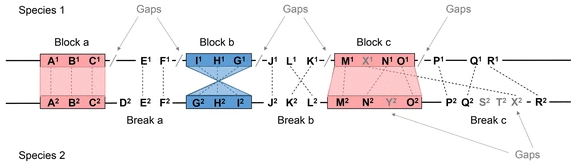
\includegraphics[width=0.7\linewidth]{../Figures/Synteny_block_definition.png}
        \vspace{-2\baselineskip}
        \caption*{\small\textbf{1 pav. Sintenijos blokų tipai}}
        %\href{https://bmcbioinformatics.biomedcentral.com/articles/\
        %10.1186/s12859-018-2026-4}{\emph{Inferring synteny between genome assemblies:
        %a systematic evaluation}}}}
        \label{fig:birds}
    \end{center}
\end{figure}

Paveiksle pavaizduotuose blokuose yra po tris ortologinius genus (inkarus):
\begin{enumerate}
    \item \textbf{A blokas:} blokas tarp vienoda tvarka išsidėsčiusių
    ortologinių genų;
    \item \textbf{B blokas:} blokas tarp priešinga tvarka išsidėsčiusių
    ortologinių genų;
    \item \textbf{C blokas:} blokas tarp ortologinių genų, kuriuos skiria
    neortologiniai genai.
\end{enumerate}

Sintenijos blokų paieška leidžia tirti skirtingų organizmų sąsajas ir genomų
evoliuciją, vykstant genomų persitvarkymo procesams. Atliekant šių blokų analizę
galima rekonstruoti filogenetinius ir filogenominius medžius\cite{PHYLO_REF},
siekiant išsiaiškinti bendrą tiriamų organizmų kilmę. Taip pat konservatyvių
genų blokų nustatymas tarp skirtingų organizmų genomų gali indikuoti funkcines
genų produktų (baltymų) sąsajas\cite{FUNC_REF}.

\newpage

\subsection{Identifikavimo metodai}
Internete galima rasti ne vieną įrankį, leidžiantį vizualizuoti gerai anotuotų
genomų sinteniją DNR lygmenyje (pavyzdžiui, Ensembl SyntenyView\cite{ENS_SYN},
NCBI MapViewer\cite{NCBI_MAP}, Genomicus\cite{GENOMICUS}), tačiau nepaisant to,
kad taikant šiuos įrankius konservatyvius regionus galima vizualizuoti ne vienu
būdu, įrankiai pateikia iš anksto suskaičiuotus rezultatus. Naudojant šiuos
įrankius tyrėjai negali pasirinkti parametrų, pavyzdžiui, leidžiančių keisti
sintenijos blokų ilgį ar minimalų genų skaičių bloke.

Dėl šių įrankių trūkumų yra sukurta daug įvairių programinių įrankių,
leidžiančių atlikti pastarųjų blokų paiešką savarankiškai, tiriant nemodelinių
organizmų genomų evoliuciją bei keičiant algoritmų parametrus. Šiuos įrankius
galima pasirinkti pagal tai, koks yra organizmų giminingumas, koks genomo
tyrimas yra atliekamas ir kokią hipotezę siekiama patvirtinti arba paneigti.

Antrame paveiksle (2 pav.) pateiktoje schemoje vaizduojami sintenijos nustatymo
metodai išskaidyti pagal lyginamų genomų giminingumą:

\begin{figure}[htb]
    \begin{center}
        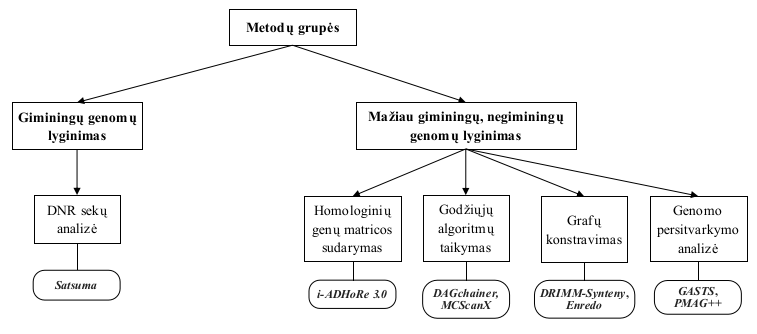
\includegraphics[width=0.9\linewidth]{../Figures/Methods_tools.png}
        \vspace{-2\baselineskip}
        \caption*{\small\textbf{2 pav. Sintenijos blokų identifikavimo
        metodai ir populiariausių įrankių pavyzdžiai}}
        \label{fig:birds}
    \end{center}
\end{figure}

\subsubsection{Giminingų organizmų genomų lyginimas}
Lyginant genomus, priklausančius itin giminingiems organizmams, sintenijos
blokai gali būti identifikuojami taikant įrankius, paremtus DNR sekų
išlyginimais, nes genomų sekų atitikimo laipsnis yra didelis (didelė dalis
nukleotidų sutampa).

Konservatyvių chromosomų regionų nustatymui naudojami DNR sekų išlyginimu
paremti metodai yra intuityvūs, tačiau reikalaujantys didelių kompiuterio
resursų (jeigu tarpusavyje lyginami eukariotinių organizmų genomai). Nepaisant
to, yra sukurta įrankių, kurie efektyviai sprendžia ne tik kompiuterio resursų
naudojimo problemą, bet ir pateikia patikimus rezultatus, leidžiančius daryti
išvadas apie atliktą tyrimą.

\subsubsection{Mažai giminingų arba negiminingų organizmų genomų lyginimas}
Tiriant tos pačios biologinės klasifikacijos taksonominio rango - klasės -
organizmus, kurie kilę iš bendro protėvio ir turi panašią sandarą, metodai, 
kurie remiasi DNR sekų išlyginimu, negali būti taikomi, nes lyginamų organizmų
DNR sekos yra pakitusios (evoliucijos eigoje įvyko daugiau įvairių mutacijų),
todėl sintenijos blokų paieška turi būti atliekama aminorūgščių lygyje.
Nepaisant evoliucijos eigoje vykstančių DNR sekų pokyčių, viena aminorūgštis
gali būti koduojama keliais skirtingais kodonais. Dėl šios priežasties metodo
taikymas tinka evoliucijos eigoje mutavusių mažai giminingų organizmų genomų
sekų lyginimui ir homologinių regionų paieškai.

Norint palyginti skirtingoms taksonominėms klasėms priklausančių organizmų
genomus taikomi metodai, analizuojantys baltymus koduojančias aminorūgštis,
bei metodai, konstruojantys profilius, grafus ir naudojantys įvairius
statistinius modelius.

Taikant šiuos metodus yra svarbu, kad analizuojamų organizmų genomai būtų kuo
kokybiškesni: jeigu genome trūksta sekų, gali nebūti tam tikrų genų anotacijų,
todėl homologinių sąsajų taip pat nebūtų galima tyrinėti - kai kurie sintenijos
blokai būtų neidentifikuoti.

\subsubsection*{Homologinių genų matricos sudarymo metodas}
Taikant šį metodą sintenijos blokai identifikuojami, naudojant kaimyninių genų
porų klasterizavimą. Genomų genų atitikimai arba neatitikimai fiksuojami
matricoje. Jeigu genai homologiniai, matricoje įrašomas '1', jei nehomologiniai
- įrašomas '0'. Remiantis šiuo metodu sintenijos blokai nustatomi, ieškant,
kurioje matricos diagonalės vietoje yra didžiausia vienetų sankaupa.

\textbf{Metodo privalumas:} taikant šį metodą nustatytiems sintenijos blokams
galima paprastai pritaikyti statistinę validaciją ir aptikti
\emph{false positive} reikšmes.

\textbf{Metodo trūkumai:} taikant šį metodą yra svarbu tiksliai žinoti, į kokį
biologinį klausimą norima atsakyti, nes nuo to priklauso, koks paieškai
reikalingas parametras arba jų konfigūracijos bus pasirinktos, jog būtų gauti
optimalūs rezultatai. Pavyzdžiui, tarpo tarp dviejų genų dydis, kuris gali
egzistuoti identifikuotame sintenijos bloke. Kuo šio parametro vertė mažesnė,
tuo daugiau nedidelių ir sunkiai analizuojamų sintenijos blokų bus nustatyta,
tačiau, jei tarpo ilgio parametro reikšmė didelė, nustatytas blokas bus didelis
- analizės atlikimas taps paprastesniu. Kita vertus, tokiame bloke gali
atsirasti tokių sekų fragmentų, kurie iš tiesų neturėtų priklausyti blokui
(daugiau \emph{false positive} reikšmių), nes nėra aptinkami kitame genome.

\subsubsection*{Godžiųjų algoritmų taikymo metodas}
Realizuojant šį metodą yra konstruojamos kolinearių genų porų grandinės. Metodo
įgyvendinimui atliekama daug daugiau skaičiavimų nei aprašytas homologinių genų
matricos sudarymo metodas.
Įrankiuose, kurie remiasi šiuo metodu, yra naudojami \emph{BLASTP} rezultatai.
Jais remiantis galima taikyti dinaminį programavimą ir sukonstruoti kolinearių
genų porų grandines, turinčias maksimalias grandinės vertes (angl. 
\emph{chainscore}). Taikant šį metodą sintenijos blokus sudaro kolineariose
pozicijose esančių unikalių homologinių sekų (sintenijos inkarų) genai bei tarp
jų išsidėstę nehomologiniai genai, kurie evoliucijos eigoje buvo paveikti
mutacijų.

\textbf{Metodo privalumai:} Taikant šį metodą galima lyginti daug skirtingų
genomų ir analizuoti genų pokyčius chromosomose. Taip pat genomų kolinearių
genų paieškos algoritmai veikia itin sparčiai ir pateikia išsamius rezultatus.

\textbf{Metodo trūkumas:} Taikant metodą reikia iš anksto žinoti, ko reikia
ieškoti, bei, kokios yra tiriamų genomų bei sintenijos blokų charakteristikos.

\subsubsection*{Grafų konstravimo metodas}
Kai yra žinomos baltymus koduojančių genų pozicijos ir sekų išlyginimo tikimybė,
galima konstruoti grafus, surenkančius visas įmanomas homologinių genų poras
tarp lyginamų genomų.

Iš pradžių yra atliekamas lokalus genomų išlyginimas, po kurio gauti išlyginimai
naudojami grafo konstravimui bei genomų vidinių struktūrų paieškai. Priklausomai
nuo to, kokį grafą bus pasirinkta konstruoti, gali būti gauti labai skirtingi
identifikuotų sintenijos blokų rezultatai. Taikant šį metodą galima konstruoti
keturių skirtingų tipų grafus: išlyginimų, \emph{de-Bruijn}, \emph{Enredo},
\emph{Cactus}.

Taikant skirtingus grafų tipus tiriamos vidinės genomo struktūros, jog būtų
identifikuoti sintenijos blokai. Šiomis struktūromis gali būti: iš eilės
einantys ir tarp dviejų genomų sutampantys genų sekų blokai, tarp kurių nėra
tarpų ir kuriems būdinga vienoda kryptis abiejuose genomuose; mikroblokai -
blokai, tarp kurių gali būti tarpų; trumpi ciklai, kurie įrodo, kad genomas
pakito, vykstant persitvarkymo procesams.

\newpage

%%%%%%%%%%%%%%%%%%%%%%%%%%%%%%%%%%%%%%%%
% KONKREČIŲ ĮRANKIŲ VEIKIMO APRAŠYMAI
%%%%%%%%%%%%%%%%%%%%%%%%%%%%%%%%%%%%%%%%

\section{Taikytų įrankių metodų aprašymai}
\subsection{\emph{Cinteny} įrankis}
Siekiant efektyviai reprezentuoti linijinę genomų markerių tvarką šiame įrankyje
implementuota išplėsta trejetainio paieškos medžio struktūra (angl.
\emph{ternary search tree} (TST)). Ši struktūra išplėsta, pavaizdavus 
„perėjimus“ tarp medžio lapų. Šie „perėjimai“ atitinka linijinius genomo
markerių „perėjimus“. Šie markeriai gali būti apibūdinti kaip ortologiniai
(homologiniai) genai.

\begin{figure}[htb]
    \begin{center}
        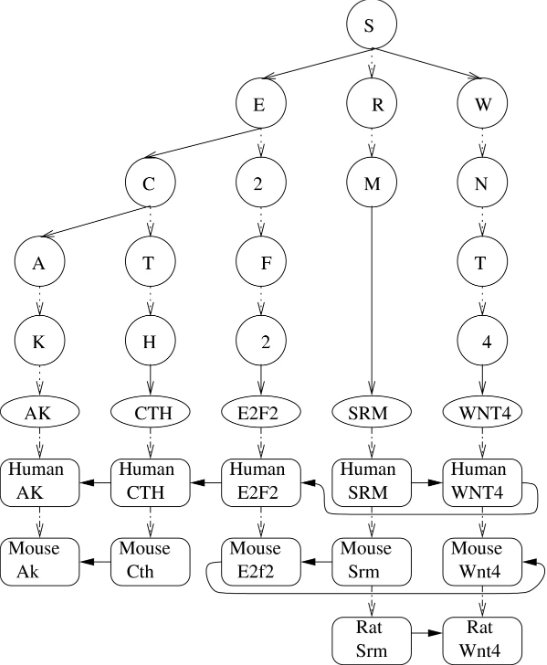
\includegraphics[width=0.4\linewidth]{../Figures/TTS_data_structure.png}
        \vspace{-0.5\baselineskip}
        \caption*{\small\textbf{4 pav. TST medžio struktūra su perėjimais}}
        \label{fig:birds}
    \end{center}
\end{figure}

Pateiktame paveiksle pavaizduota TST medžio struktūra su „perėjimais“ keliems
genams iš žmogaus, pelės ir žiurkės genomų. Paveiksle viršūnės (apskritimai)
atitinka genų simbolius, medžio lapai (elipsės) atitinka homologinę grupę.
Individualūs genai (meta viršūnės), priklausantys kiekvienai homologinei grupei,
atvaizduoti po medžio lapais. Linijiniai perėjimai sukonstruoti, sujungus meta
viršūnes ta tvarka, kuria genai nustatyti chromosomose.

Konservatyvių genų blokai, išlaikantys savo eiliškumą, yra agreguojami į
didesnius blokus, neįtraukiant blokų, kurie gauti atlikus sekų
mikropertvarkymus. Keičiant įrankio parametrus (minimalų sintenijos blokų
ilgį, maksimalų tarpą tarp agreguotų blokų ir minimalų genų - markerių - skaičių
bloke) gali būti gauti skirtingi sintenijos blokai.

Šios hibridinės struktūros taikymas leidžia atlikti genų paiešką per logaritminį
laiką, įvardinti visus galimus ortologus bei pereiti visus genų perėjimus iš 5'
galo link 3' chromosomos galo arba atvirkščiai. Struktūrą realizuojantis
algoritmo kompleksiškumas yra $ N\log_{10}N $, kur N skaičius nurodo genome
nustatytų genų skaičių, todėl šį metodą galima taikyti ir dideliems genomams.

\newpage

%%%%%%%%%%%%%%%%%%%
% TYRIMO METODAI
%%%%%%%%%%%%%%%%%%%

\section{Tyrimo metodai}
Homologijos tarp \emph{Mus musculus} ir \emph{Danio rerio} organizmų
tyrimo analizė atlikta su R programavimo kalba\cite{R} (4.2.2 versija)

Tarpiniai analizės rezultatai pateikti, naudojant komandinės eilutės įrankį
Scikick\cite{SCIK} (0.2.0 versija). Naudojant šį įrankį buvo apjungti keli Rmd
failai ir gauta HTML formato ataskaita \hyperref[Priedas]{(6 skyriaus priedas)}.

\subsection{Sintenijos blokų nustatymas ir vizualizavimas}
Sintenijos blokai tarp \emph{Mus musculus} ir \emph{Danio rerio} organizmų
nustatyti ir vizualizuoti pasinaudojus internetinės
\emph{Synteny Portal}\cite{SYN_PORT} aplikacijos \emph{SynCircos} įrankiu.

\subsection{Sintenijos blokų pozicijų gavimas}
Šiame analizės etape sintenijos blokai buvo gauti pasinaudojus Cinteny
įrankiu, kurio pateiktoje išvestyje buvo nurodytos pirmojo genomo
\emph{Mus musculus} genominės pozicijos ir antrojo genomo \emph{Danio rerio}
genominės pozicijos, kuriose abiejų genomų sekų fragmentai sutapo - gauti
sintenijos blokai.

\subsection{Pikų persidengimas su sintenijos blokais}
Sintenijos blokų failas buvo apdorotas R programoje, kurioje apskaičiuota
kiekvieno mėginio pikų bei su sintenijos blokais persidengiančių pikų dalis,
panaudojus \emph{rtracklayer}\cite{R_TRACK} bibliotekos funkciją
\emph{subsetByOverlaps()}. Stulpelinės diagramos sukurtos su
\emph{ggplot2}\cite{R_GGPLOT} bibliotekos \emph{geom\_bar()} funkcija.

\subsection{Pikų anotavimas}
Analizuotų mėginių pikai anotuoti (apskaičiavus atstumą iki transkripcijos
pradžios regiono (angl. \emph{\textbf{T}ranscription \textbf{S}tart
\textbf{S}ite}) ir pikams priskyrus artimiausius genus), pasinaudojus R
programavimo kalbos bibliotekos \emph{ChIPseeker}\cite{CHIP1, CHIP2} funkcija
\emph{annotatePeak()}. Dveji iš šiai funkcijai perduotų parametrų buvo gauti
įdiegus \emph{TxDb.Mmusculus.UCSC.mm10.knownGene}\cite{KNOWN_GENE} (visų žinomų
\emph{Mus musculus} genų rinkinį) ir \emph{org.Mm.eg.db}\cite{MM_ANNOT}
bibliotekas.

\subsection{Sintenijos blokams priklausančių genų nustatymas}
Sintenijos blokams priklausančių \emph{Danio rerio} genų nustatytymui panaudota
\emph{dataframe} duomenų struktūra. Ši struktūra gauta, pasinaudojus
\emph{genes()} funkcija, kuriai perduotas visų žinomų \emph{Danio rerio} genų
pozicijų ir kitos informacijos apie genus objektas
\emph{TxDb.Drerio.UCSC.danRer11.refGene}. Gautam genų duomenų rinkiniui
pritaikyta \emph{mapIds()} funkcija, kuri kiekvienam genui priskyrė atitinkamą
geno simbolį, remiantis žinomu \emph{EntrezID} identifikatoriumi iš
\emph{org.Dr.eg.db} bibliotekos objekto.

Nustačius visų žinomų zebražuvės genų simbolius, nustatyta, kurie genai sutampa
su \emph{Mus musculus} genais, pasinaudojus standartinės R bibliotekos
\emph{dplyr} funkcijomis. Gautas mažesnis genų rinkinys perduotas bibliotekos
\emph{GenomicRanges} funkcijai \emph{subsetByOverlaps()}, grąžinančiai
\emph{GRanges} objektą su pozicijomis ir anotacijomis, kurios patenka į
sintenijos blokų genominius intervalus.

\subsection{Transkripcijos faktoriaus prisijungimo sričių nustatymas}
Šiame analizės etape sudarytos dvi atskiros duomenų struktūros, kuriose
išsaugota informacija apie \emph{Mus musculus} ir \emph{Danio rerio} genus,
kurie sutampa tarp analizuojamų organizmų ir priklauso žinomiems sintenijos
blokams, specifikuojant genų simbolius ir jų pozicijas.

Turint abiejų genomų sutampančių genų objektus, panaudota \emph{Biostrings}
bibliotekos funkcija \emph{getSeq()}, kuriai buvo perduoti analizuojamo genomo
\emph{BSenome} klasės objektai (\emph{BSgenome.Mmusculus.UCSC.mm10} ir
\emph{BSgenome.Drerio.UCSC.danRer11}) bei genų pozicijų GRanges objektai.
Funkcija grąžino pozicijas atitinkančias nukleotidų sekas.

Siekiant įvertinti, ar lyginamų naminės pelės ir zebražuvės genomų sekose gali
prisijungti kardiogeninis Tbx5 transkripcijos faktorius, buvo skaičiuojami Tbx5
transkripcijos faktoriaus pozicinės svorių matricos (PWM) atitikimai sekose,
naudojant funkciją \emph{countPWM()}. Pozicinė svorių matrica atsisiųsta iš
iš HOCOMOCO[17] (11.0 versija) duomenų bazės \emph{Homo sapiens} ir
\emph{Mus musculus} organizmų transkripcijos faktorių kolekcijos.

Kiekvieno organizmų geno PWM matricos atitikimai vizualizuoti taškine diagrama,
pritaikius \emph{ggplot} funkciją \emph{geom\_point()}.

\newpage

%%%%%%%%%%%%%%%%%%%%%%%%%%%%%%%
% REZULTATAI IR JŲ APTARIMAS
%%%%%%%%%%%%%%%%%%%%%%%%%%%%%%%

\section{Rezultatai ir jų aptarimas}
\subsection{Sintenijos blokų nustatymas ir vizualizavimas}

Sintenijos blokai tarp \emph{Mus musculus} ir \emph{Danio rerio} organizmų
genomų vizualizuoti \emph{circo} diagramoje (3 pav.).

\begin{figure}[htb]
    \begin{center}
        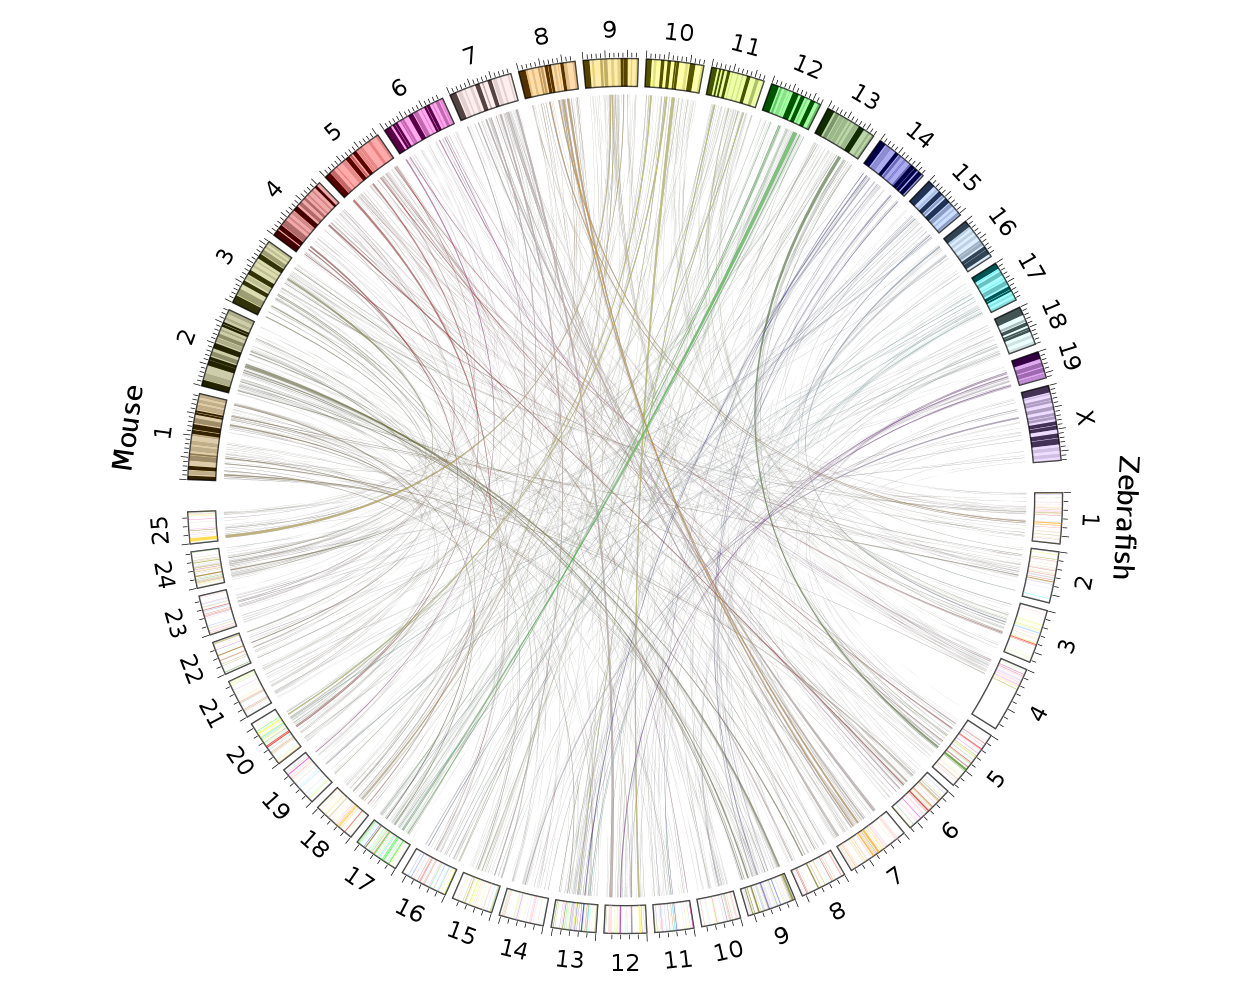
\includegraphics[width=0.8\linewidth]{../Figures/SynCircos.png}
        \vspace{-1\baselineskip}
        \caption*{\small\textbf{3 pav. Sintenijos blokų \emph{circo}
        diagrama}}
        \label{fig:birds}
    \end{center}
\end{figure}

Remiantis sukurta diagrama, galima pastebėti, kad tarp viso naminės pelės
chromosomų rinkinio nebuvo nei vienos chromosomos, kurios fragmentai nebūtų
nustatyti zebražuvės genome. Nepaisant to, naminės pelės fragmentų
pozicijos akivaizdžiai nesutapo su zebražuvės genome nustatytomis tų pačių
arba evoliucijos eigoje mutavusių fragmentų pozicijomis (naminės pelės
fragmentai buvo nustatyti kitose zebražuvės chromosomose).

Zebražuvės genome nustatytas ne vienas homologiškai su naminės pelės genomu
susijęs fragmentas, tačiau ketvirtoje zebražuvės chromosomoje (remiantis
NCBI\cite{NCBI} duomenimis tai yra didžiausia \emph{Danio rerio} chromosoma,
kurią sudaro 78,093,715 bazių poros) sintenijos blokų sankaupa pastebima
tik vienoje chromosomos pusėje (pavienių blokų nenustatyta).

\subsection{Sintenijos blokų pasiskirstymas chromosomose}
Pateiktoje diagramoje vaizduojama, kiek kiekvienos naminės pelės chromosomos
fragmentų buvo nustatyta skirtingose zebražuvės chromosomose bei pozicijose,
neatsižvelgus į sekų fragmentų ilgį.

\begin{figure}[htb]
    \centering
    \begin{subfigure}[b]{0.45\textwidth}
        \centering
        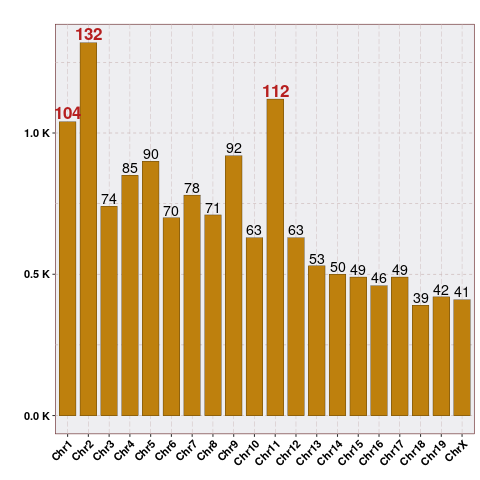
\includegraphics[width=\textwidth]{../Figures/Synteny_Chr_MM.png}
        \caption*{\centering\small\textbf{a) Fragmentų skaičius \emph{Mus musculus} chromosomose}}
    \end{subfigure}
    \hfill
    \begin{subfigure}[b]{0.45\textwidth}
        \centering
        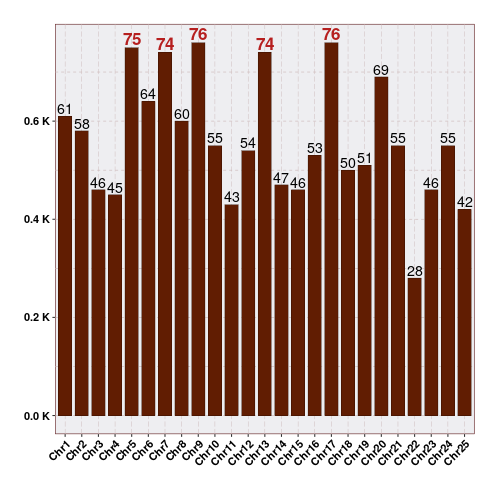
\includegraphics[width=\textwidth]{../Figures/Synteny_Chr_DR.png}
        \caption*{\centering\small\textbf{b) Fragmentų skaičius \emph{Danio rerio} chromosomose}}
    \end{subfigure}
    \caption*{\small\textbf{4 pav. Sekų fragmentų pasiskirstymas chromosomose}}
    \label{fig:birds}
\end{figure}

Pateiktoje stulpelinėje diagramoje išsiskiria trys chromosomos (\emph{Chr1},
\emph{Chr2} ir \emph{Chr11}). Šių naminės pelės chromosomų fragmentai
pasitaikydavo zebražuvės genome dažniausiai. Atsižvelgus į šių chromosomų
dydžius, kur vienuolikta chromosoma yra mažesnė nei kitos išskirtos chromosomos
(ją sudaro 122 Mbp\cite{MGI}), buvo nustatyta sąlyginai didelė dalis fragmentų,
turinčių homologijų su zebražuvės genomo sekų fragmentais.

Patikrinus, kiek yra \emph{Danio rerio} chromosomų fragmentų, kurie patenka į
sintenijos blokus, gauti rezultatai vizualizuoti ketvirto paveikslo b) dalyje.
Galima pastebėti, kad sintenijos blokams priklausančių chromosomų fragmentų
skaičius buvo itin nevienodas, palyginus su \emph{Mus musculus} rezultatais.
Chromosomose, kuriose esantys fragmentai buvo dažniausiai homologiški naminės
pelės genomui (\emph{Chr9} ir \emph{Chr17}), buvo nustatyta po 76 sintenijos
blokui priklausančius fragmentus. Mažiausias sintenijos blokui priklausančių
fragmentų skaičius nustatytas 22 chromosomoje (28 fragmentai).

\newpage

\subsection{Sintenijos blokų dalis pikuose}
\emph{Cinteny} įrankio pateikta sintenijos blokų informacija buvo panaudota,
siekiant išsiaiškinti, kokia pikų dalis patenka į įrankio nustatytų sintenijos
blokų intervalus, kurių buvo nustatyta 1403. Penktame paveiksle (5 pav.)
pavaizduota, kiek kiekviename analizuotame naminių pelių širdžių ląstelių
mėginyje nustatyta pikų, kurie patenka į sintenijos blokų intervalą.

\begin{figure}[htb]
    \begin{center}
        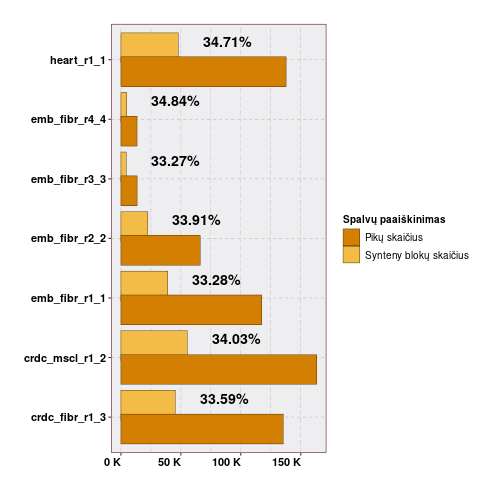
\includegraphics[width=0.8\linewidth]{../Figures/Synteny_blocks_peaks.png}
        \vspace{-2\baselineskip}
        \caption*{\small\textbf{5 pav. Sintenijos blokų procentinė dalis}}
        \label{fig:birds}
    \end{center}
\end{figure}

Remiantis gautu rezultatu galima pastebėti, kad didžiausias nustatytų sintenijos
blokų skaičius (34.84\%), palyginus su bendru pikų skaičiumi, būdingas
\emph{emb\_fibr\_r4\_4} mėginiui, kuriame naminių pelių embrionų fibroblastų
ląstelės buvo veiktos tik Tbx5 kardiogeniniu transkripcijos faktoriumi.
Mažiausias sintenijos blokų skaičius (33.27\%) nustatytas
\emph{emb\_fibr\_r3\_3} mėginyje, kuriame pelių embrionų fibroblastų ląstelės
veiktos GATA4, MEF2C ir Tbx5 transkripcijos faktoriaus, ir mėginyje
\emph{emb\_fibr\_r1\_1}, kur embrionų fibroblastai veikti pilnu kargdiogeninių
transkripcijos faktorių komplektu (AHGMT) (33.28\%). Nepaisant to, kad
pastaruosiuose mėginiuose bendras pikų skaičius skyrėsi daug, bendras sintenijos
blokams priklausančių pikų procentas skyrėsi vos 0.01\%.

Apibendrinus visus gautus mėginių rezultatus galima daryti išvadą, kad visiems
mėginiams būdingas panašus skaičius pikų, kurie priklauso sintenijos blokams,
todėl turint šią informaciją galima detaliau tyrinėti pikus, priklausančius
blokams.

\subsection{Pikų anotavimas}
\subsubsection{Artimiausių TSS nustatymas}
Šeštame paveiksle pavaizduotoje diagrama nurodyta, kiek unikalių genų buvo
priskirta kiekvieno mėginio pikams, patenkantiems į sintenijos blokus.

\begin{figure}[htb]
    \begin{center}
        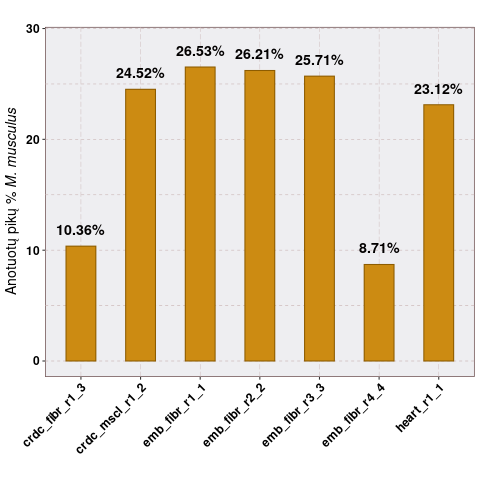
\includegraphics[width=0.7\linewidth]{../Figures/Unique_genes_MM.png}
        \vspace{-2\baselineskip}
        \caption*{\small\textbf{6 pav. Anotuotų pikų dalis mėginiuose}}
        \label{fig:birds}
    \end{center}
\end{figure}

Remiantis diagramos duomenimis pastebėta, kad daugiausiai unikalių genų
nustatyta \emph{emb\_fibr\_r1\_1} mėginyje (26.53\%). Ankstesniame paveiksle
(5 pav.) šiame mėginyje buvo nustatyta nedaug sintenijos blokams priklausančių
pikų, tačiau nebuvo atsižvelgta į sintenijos blokų ilgį. Gautas rezultatas rodo,
kad pikai galėjo patekti į ilgesnį sintenijos bloką.

Mažiausiai unikalių genų nustatyta \emph{emb\_fibr\_r4\_4} mėginyje (8.71\%).
Rezultatas gali rodyti, kad pikai priklausė didesniam sintenijos blokų skaičiui,
tačiau blokai buvo trumpi.

\subsubsection{Genominių elementų pasiskirstymas}
Anotuojant mėginių sintenijos blokams priklausančius pikus taip pat buvo
nustatyta, kokiems genominiams elementams priklauso kiekvienas pikas. Antroje
lentelėje (lentelė 2) išskirti genominiai elementai, kuriems priklauso
didžiausias procentas anotuotų mėginių pikų. Kitiems genominiams elementams
(5' ir 3' sritims, promotoriams nuo 1 iki 2 kb ir nuo 2 iki 3 kb, egzonams)
priklausė mažiau nei 7\% visų mėginių pikų, todėl jie neanalizuoti.

\begin{table}[htb]
    \newcolumntype{M}[1]{>{\centering\arraybackslash}m{#1}}
    \small
    \caption*{\small\textbf{2 lentelė. Genominių elementų procentinė dalis
                            mėginiuose}}
    \begin{tabular}{|c|c|c|c|c|}
        \hline
        \textbf{\thead{Mėginys}} & \textbf{\thead{Promotorius (<=1kb)}} &
        \textbf{\thead{Pirmas intronas}} & \textbf{\thead{Kiti intronai}} &
        \textbf{\thead{Tarpgeninė sritis}} \\
        \hline
        \textbf{\thead{\emph{crdc\_mscl\_r1\_2}}} & 21.31\% & 12.72\% &
                24.18\% & 19.65\% \\
        \hline
        \textbf{\thead{\emph{emb\_fibr\_r1\_1}}} & 13.69\% & 15.09\% &
                31.61\% & 24.69\% \\
        \hline
        \textbf{\thead{\emph{emb\_fibr\_r2\_2}}} & 16.91\% & 13.67\% &
                30.5\% & 26.19\% \\
        \hline
        \textbf{\thead{\emph{emb\_fibr\_r3\_3}}} & 18.65\% & 13.08\% &
                30.2\% & 25.45\% \\
        \hline
        \textbf{\thead{\emph{heart\_r1\_1}}} & 27.97\% & 11.54\% &
                26.7\% & 21.97\% \\
        \hline
        \textbf{\thead{\emph{emb\_fibr\_r4\_4}}} & 6.49\% & \textbf{16.34\%} &
                \textbf{36.73\%} & \textbf{28.37\%} \\
        \hline
        \textbf{\thead{\emph{crdc\_fibr\_r1\_3}}} & \textbf{30.83\%} & 12.06\% &
                24.88\% & 20.12\% \\
        \hline
    \end{tabular}
\end{table}

Remiantis lentelės duomenimis \emph{emb\_fibr\_r4\_4} didžioji mėginio pikų
dalis priklausė introninėms ir tarpgeninėms sritims, naminių pelių embrionų
fibroblastų ląsteles paveikus tik Tbx5 transkripcijos faktoriumi. Be to, šiame
mėginyje nustatytas itin mažas procentas pikų, priklausančių promotorinėms
sritims. Atsižvelgus į tai, kad to paties eksperimento mėginiai, kuriems taikyti
skirtingi poveikiai, galima daryti išvadą, kad genominių elementų pasiskirstymo
procentas priklauso nuo to, kokiais poveikiais veikiamos naminės pelės ląstelės.

\newpage

\subsection{Genų nustatymas zebražuvėje}
Turint duomenis apie homologiškas sritis tarp \emph{Mus musculus} ir
\emph{Danio rerio} organizmų buvo patikrinta, kurie anotuoti kiekvieno naminės
pelės pikų mėginių genai priklauso ir zebražuvės genų rinkiniui, bei kiek šių,
tarp organizmų sutampančių, genų gali būti nustatyta zebražuvės sintenijos
blokams priklausančiose pozicijose. Gauti rezultatai pateikti žemiau esančiame
paveiksle.

\begin{figure}[htb]
    \begin{center}
        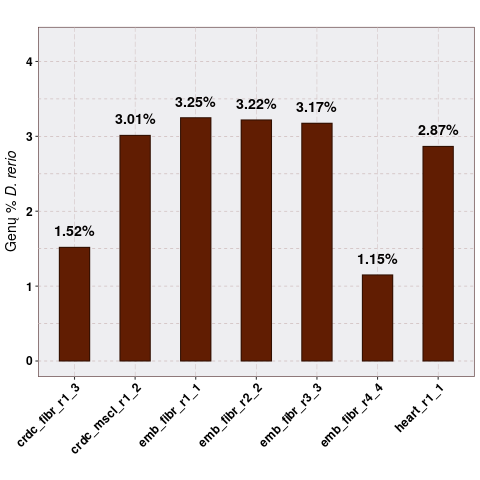
\includegraphics[width=0.7\linewidth]{../Figures/Unique_genes_DR.png}
        \vspace{-2\baselineskip}
        \caption*{\small\textbf{6 pav. D.rerio sintenijos blokams priklausančių
        genų dalis}}
        \label{fig:birds}
    \end{center}
\end{figure}

Remiantis gauta diagrama galima pastebėti, kad zebražuvės genų, sutampančių su
naminės pelės genais ir priklausančių sintenijos blokams, buvo itin nedaug.
Palyginus visus mėginių anotuotų pikų genų rinkinius su zebražuvės genų rinkiniu
bendrų genų dalis buvo mažesnė nei 4\%.

\subsection{Transkripcijos faktoriaus prisijungimas zebražuvės sekose}
Nepaisant mažo bendrų genų tarp \emph{Mus musculus} ir \emph{Danio rerio}
organizmų buvo patikrinta, ar zebražuvės pozicijose, patenkančiose į sintenijos
blokus, gali jungtis Tbx5 transkripcijos faktorius. Sekų fragmentų,
atitinkančių Tbx5 pozicinę svorių matricą, skaičius palygintas su atitikimų
skaičiumi, gautu Tbx5 transkripcijos faktoriaus pozicinę svorių matricą
pritaikius naminės pelės sintenijos blokams priklausančioms sekoms.

Žemiau pateikiamame paveiksle vaizduojamas Tbx5 transkripcijos faktoriaus
matricos atitikimas \emph{Mus musculus} ir \emph{Danio rerio} sekose.

\begin{figure}[htb]
    \begin{center}
        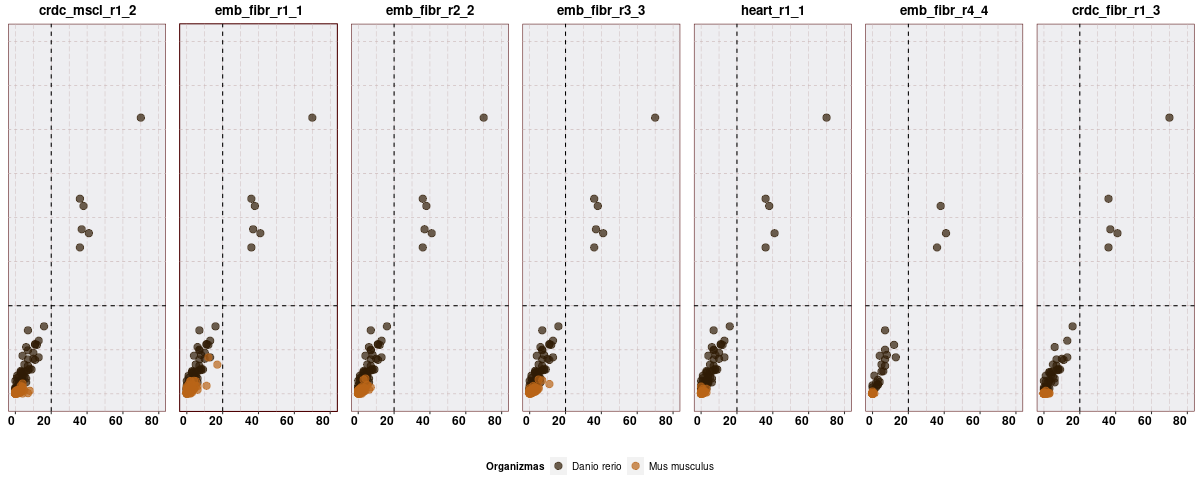
\includegraphics[width=1\linewidth]{../Figures/PWM_matches_all.png}
        \vspace{-2\baselineskip}
        \caption*{\small\textbf{7 pav. PWM matricos atitikimai M.musculus ir
        D.rerio sekose}}
        \label{fig:birds}
    \end{center}
\end{figure}

Palyginus gautus rezultataus galima pastebėti, kad visais atvejais pozicinės
matricos atitikimas \emph{Danio rerio} sekoms buvo panašus. Zebražuvės genome
buvo genų, kurių dydis viršijo 100000 nukleotidų (taškai, priklausantys I
ketvirčiui). Šiose sekose Tbx5 pozicinės svorių matricos atitikimų buvo
nustatyta daugiau nei 30.

Naminės pelės genuose PWM matricos atitikimų buvo nustatyta mažiau. Be to, sekų
ilgis buvo mažesnis. Mėginyje \emph{emb\_fibr\_r4\_4} Tbx5 pozicinės svorių
matricos anotuotų pikų genų atitikimų buvo mažiausiai, todėl tikėtina, kad šiame
mėginyje Tbx5 transkripcijos faktorius jungtųsi retai.

\subsection{Sintenijos blokams priklausančių genų biologinės funkcijos}
\emph{Danio rerio} genams, priklausantiems sintenijos blokams ir sutampantiems
su \emph{Mus musculus} genais, atlikta biologinių funkcijų nustatymo analizė.
Gautos biologinės funkcijos pateiktos žemiau esančioje lentelėje?

%%%%%%%%%%%%%%%%%%%%%
% SYMAP REZULTATAS
%%%%%%%%%%%%%%%%%%%%%

%\subsection*{\textbf{Symap} įrankis}
%Šioje analizėje buvo panaudotas įrankis \emph{Symap}\cite{SYMAP}, kurio
%rezultatas palygintas su rezultatais, gautais taikant kitus metodus
%realizuojančius įrankius. Šio metodo rezultatas pateiktas 5 pav. 


% Apibendrinus gautus rezultatus nustatyta sintenijos blokų dalis
% pikų atžvilgiu buvo maža (neviršijo 20\%), todėl sintenijos blokų paieška
% nėra tinkamiausias būdas, siekiant įvertinti \emph{Mus musculus} ir
% \emph{Danio rerio} organizmų homologiją, nes taikomas sintenijos blokų
% paieškos metodas, tikėtina, nesuranda visų galimų homologiškų
% \emph{Mus musculus} ir \emph{Danio rerio} organizmų genomų fragmentų.

\newpage

%%%%%%%%%%%%
% IŠVADOS
%%%%%%%%%%%%

\section{Išvados}

\newpage

%%%%%%%%%%%%%%%
% LITERATŪRA
%%%%%%%%%%%%%%%

\bibliographystyle{plain}
\begin{thebibliography}{99}

\bibitem{GTRD} GTRD: an integrated view of transcription regulation.
Kolmykov S, Yevshin I, Kulyashov M, Sharipov R, Kondrakhin Y, Makeev VJ,
Kulakovskiy IV, Kel A, Kolpakov F Nucleic Acids Res. 2021 Jan
8;49(D1):D104-D111.

\bibitem{PHYLO_REF} Nadeau JH, Taylor BA: Lengths of chromosomal segments
conserved since divergence of man and mouse. Proc Nat Acad Sci 1984,
81: 814–818. 10.1073/pnas.81.3.814.

\bibitem{FUNC_REF} Frazer KA, Elnitski L, Church DM, Dubchak I, Hardison RC:
Cross-species comparisons: a review of methods and available resources.
Genome Res 2003, 13: 1–12. 10.1101/gr.222003.

\bibitem{ENS_SYN} Clamp M, Andrews D, Barker D, Bevan P, Cameron G, Chen Y,
Clark L, Cox T, Cuff J, Curwen V, Down T, Durbin R, Eyras E, Gilbert J,
Hammond M, Hubbard T, Kasprzyk A, Keefe D, Lehvaslaiho H, Iyer V, Melsopp C,
Mongin E, Pettett R, Potter S, Rust A, Schmidt E, Searle S, Slater G, Smith J,
Spooner W, Stabenau A, Stalker J, Stupka E, Ureta-Vidal A, Vastrik I, Birney E:
Ensembl 2002: accommodating comparative genomics. Nucleic Acids Res 2003,
31: 38–42. 10.1093/nar/gkg083.

\bibitem{NCBI_MAP} Wheeler DL, Barrett T, Benson DA, Bryant SH, Canese K,
Chetvernin V, Church DM, DiCuccio M, Edgar R, Federhen S, Geer LY, Kapustin Y,
Khovayko O, Landsman D, Lipman DJ, Madden TL, Maglott DR, Ostell J, Miller V,
Pruitt KD, Schuler GD, Sequeira E, Sherry ST, Sirotkin K, Souvorov A,
Starchenko G, Tatusov RL, Tatusova TA, Wagner L, Yaschenko E: Database
resources of the National Center for Biotechnology Information. Nucleic Acids
Res 2007, (35 Database):D5-D12. 10.1093/nar/gkl1031.

\bibitem{GENOMICUS} Matthieu Muffato, Alexandra Louis, Charles-Edouard Poisnel,
Hugues Roest Crollius, Genomicus: a database and a browser to study gene
synteny in modern and ancestral genomes, Bioinformatics, Volume 26, Issue 8,
15 April 2010, Pages 1119–1121, https://doi.org/10.1093/bioinformatics/btq079.

\bibitem{CINTENY} Sinha, A.U., Meller, J. Cinteny: flexible analysis and
visualization of synteny and genome rearrangements in multiple organisms.
BMC Bioinformatics 8, 82 (2007). https://doi.org/10.1186/1471-2105-8-82

\bibitem{ARTICLE1} Liu, D., Hunt, M. \& Tsai, I.J. Inferring synteny between
genome assemblies: a systematic evaluation. BMC Bioinformatics 19, 26 (2018).
https://doi.org/10.1186/s12859-018-2026-4

\bibitem{ARTICLE2} Lallemand, T.; Leduc, M.; Landès, C.; Rizzon, C.; Lerat, E.
An Overview of Duplicated Gene Detection Methods: Why the Duplication Mechanism
Has to Be Accounted for in Their Choice. Genes 2020, 11, 1046.
https://doi.org/10.3390/genes11091046

\bibitem{R} R Core Team (2022).
R: A language and environment for statistical computing. R Foundation
for Statistical Computing, Vienna, Austria. URL https://www.R-project.org/.

\bibitem{SCIK} Scikick. Utility for executing collections of computational
notebooks.\\
URL https://petronislab.camh.ca/pub/scikick/stable/docs/report/out\_html/introduction.html.

\bibitem{SYN_PORT} Lee J, Hong WY, Cho M, Sim M, Lee D, Ko Y, Kim J. Synteny
Portal: a web-based application portal for synteny block analysis. Nucleic
Acids Res. 2016 Jul 8;44(W1):W35-40. doi: 10.1093/nar/gkw310. Epub 2016 May 6.
PMID: 27154270; PMCID: PMC4987893.

\bibitem{R_TRACK} M. Lawrence, R. Gentleman, V. Carey: "rtracklayer: an {R}
package for interfacing with genome browsers". Bioinformatics 25:1841-1842.

\bibitem{R_GGPLOT} H. Wickham. ggplot2: Elegant Graphics for Data Analysis.
Springer-Verlag New York, 2016.

\bibitem{CHIP1} Wang Q, Li M, Wu T, Zhan L, Li L, Chen M, Xie W, Xie Z, Hu E,
Xu S, Yu G (2022). “Exploring epigenomic datasets by ChIPseeker.” Current
Protocols, 2(10), e585. doi: 10.1002/cpz1.585.

\bibitem{CHIP2} Yu G, Wang L, He Q (2015). “ChIPseeker: an R/Bioconductor
package for ChIP peak annotation, comparison and visualization.”
Bioinformatics, 31(14), 2382-2383. doi: 10.1093/bioinformatics/btv145.

\bibitem{KNOWN_GENE} Team BC, Maintainer BP (2019).
TxDb.Mmusculus.UCSC.mm10.knownGene: Annotation package for TxDb object(s).
R package version 3.10.0.

\bibitem{MM_ANNOT} Carlson M (2022). org.Mm.eg.db: Genome wide annotation for
Mouse. R package version 3.15.0.

\bibitem{R_TRACK} M. Lawrence, R. Gentleman, V. Carey: "rtracklayer: an {R}
package for interfacing with genome browsers". Bioinformatics 25:1841-1842.

\bibitem{HOCOMOCO} HOCOMOCO: towards a complete collection of transcription
factor binding models for human and mouse via large-scale ChIP-Seq analysis
Ivan V. Kulakovskiy; Ilya E. Vorontsov; Ivan S. Yevshin; Ruslan N. Sharipov;
Alla D. Fedorova; Eugene I. Rumynskiy; Yulia A. Medvedeva; Arturo Magana-Mora;
Vladimir B. Bajic; Dmitry A. Papatsenko; Fedor A. Kolpakov; Vsevolod J. Makeev
Nucl. Acids Res., Database issue, gkx1106 (11 November 2017)
doi: 10.1093/nar/gkx1106.

\bibitem{NCBI} National Center for Biotechnology Information (NCBI)[Internet].
Bethesda (MD): National Library of Medicine (US), National Center for
Biotechnology Information; [1988] – [cited 2023 Jan 22]. Available from:
https://www.ncbi.nlm.nih.gov/

\bibitem{MGI} Bult CJ, Blake JA, Smith CL, Kadin JA, Richardson JE, the
Mouse Genome Database Group. 2019. Mouse Genome Database (MGD) 2019.
Nucleic Acids Res. 2019 Jan. 8;47 (D1): D801–D806.
\end{thebibliography}

\newpage

%%%%%%%%%%%%
% PRIEDAI
%%%%%%%%%%%%

\section{Priedas} \label{Priedas}

Priedų sąraše pateikiamos tarpinių rezultatų puslapio, sugeneruoto su Scikick,
bei Git repozitorijos, kurioje saugomi analizei naudoti duomenų failai,
parašyti skriptai bei pagrindinė R programa, nuorodos.

\begin{itemize}
    \item \textbf{Kursinio projekto analizės Git repozitorija:}\\
        \url{https://github.com/dansta0804/Tbx5\_analysis\_II.git}
    \item \textbf{Kursinio darbo Scikick ataskaita:}\\
        \url{https://karklas.mif.vu.lt/\string~dast6577/KursinisDarbas/v2.0/peaks\_MM.html}
    \item \textbf{Kursinio darbo analizės Git repozitorija:}\\
        \url{https://github.com/dansta0804/Tbx5\_analysis.git}
  \end{itemize}

\end{document}